\documentclass{tfgitic}[2024/07/01]
% per a fórmules químiques
\usepackage[version=4]{mhchem}
% Per dibuixar gràfics: base general i gràfics senzills
\usepackage{tikz}
\usetikzlibrary{arrows}
% Per dibuixar gràfics: circuits electrònics
\usepackage[europeanresistors,americaninductors]{circuitikz}
% Per dibuixar gràfics: diagrames diversos
\usepackage{pgfplots}
% Per escriure algoritmes
\usepackage[plain,figure]{algorithm2e}
% Per a usar taules elàstiques
\usepackage{tabularx}





% Indica quines bd bibliografiques usarem
\addbibresource{docum-tfe.bib}

% Marges en els algoritmes
\setlength{\algomargin}{4em}

% Versió de pgfplots a usar
\pgfplotsset{compat=newest}

\definecolor{tufte1}{rgb}{0.7,0.7,0.55}
\definecolor{yellowmarker}{HTML}{DEF440}

\pgfplotsset{
  tufte bar/.style={
    ybar,
    axis line style={draw opacity=0},
    xtick=\empty,
    ymin=0,
    bar width=3mm,
    x=2*\pgfkeysvalueof{/pgf/bar width},
    ymajorgrids,
    grid style=white,
    axis on top,
    major tick length=0pt,
    cycle list={
      fill=tufte1, draw=none\\
    },
    enlarge x limits={
      abs=0.5*\pgfkeysvalueof{/pgf/bar width}
    },
    axis x line*=bottom,
    x axis line style={
      draw opacity=1,
      tufte1,
      thick
    },
    yticklabel=\pgfmathprintnumber{\tick}\,\%
  }
}



\title{
  Un exemple de TFE\\
  Composició, ortotipografia i tipografia.
}

\subtitle{Versió 7.1}

\author{Berenguer de Cruïlles}

\advisor{Sebastià Vila-Marta}



\topics{
  Memòria \acro{tfe};
  UPC Manresa
  }


\dedication{
  A les persones arrossegades
  pel maligne cap als editors \acro{wysiwyg}.\\
  Que la sort les acompanyi.
}

\begin{acknowledgments}
  El més sentit agraïment a tots els que em van empènyer a aprendre
  \TeX{} quan no era fàcil ni tan sols imprimir-ne el resultat. Ells
  em van descobrir el món de la tipografia i sempre més n'he gaudit
  amb passió.

  El meu agraïment també als estudiants i estudiantes que han fet de
  revisors d'aquesta classe usant-la en els seus treballs. Molts
  d'ells m'han fet suggeriments i crítiques valuoses que han anat
  millorant aquest estil. He procurat que el seu nom sortís reflectit
  a la història d'aquesta classe (apèndix~\ref{cap:historia}).

  Montse Méndez va fer una lectura acurada de la versió {6.4}
  d'aquesta documentació i va ajudar notablement a la seva
  millora. Tot el meu agraïment.
\end{acknowledgments}


\begin{resum}
  Aquest document i\l.lustra la «classe» \LaTeX{} \texttt{tfgitic}.
  La classe va ser dissenyada per a escriure la memòria del treball fi
  de grau de l'Enginyeria de Sistemes \acro{tic} a la Universitat
  Politècnica de Catalunya, però també es pot fer servir en altres
  titulacions de grau o màster sense cap restricció.

  La memòria sempre ha d'anar acompanyada dels resums en català i en
  anglès.
\end{resum}


\begin{abstract}
  This document illustrates the \LaTeX{} «class» \texttt{tfgitic}.
  The class was designed to write the bachelor thesis manuscript to
  fulfill the requirements of the \acro{ict} Systems Engineering
  degree at Technical University of Catalonia. However, it can be
  used in other bachelor or master degrees with no constraints.

  The abstracts written in english and catalan are mandatory sections
  of the manuscript.
\end{abstract}



\begin{document}



\part{Memòria}

\chapter{Introducció}
\label{cap:intro}

L'internet de les coses \emph{IoT} és un nombre de xarxes que permeten un intercanvi d'informació entre sistemes 
sense la intervenció del ser humà. El mercat de \emph{IoT} ha crescut significativament a causa de la seva utilitat en la indústria. 
En molts casos \emph{IoT} es presenta com una nova revolució industrial i es ven com una tecnologia
que permet crear sistemes inte\l.ligents. Relitzar sistemes inte\l.ligents com 
vehicles,ciutats,edificis etc no és una feina senzilla i es requereixen protocols força complexos.

Actualment les aplicacions de \emph{IoT} necessiten cada cop  noves tecnologies que ofereixin un consum baix, preu baix   
i complexitat baixa. En molts casos els dispositius finals són sistemes encastats formats per una bateria, sensors i 
un microcontrolador. És fonamental tenir un bon sistema per disminuir el màxim el consum del dispositiu i així augmentar
el temps de vida de la bateria. La comunicació del dispositiu pot ser de centenars de metres fins a quilòmetres.
Aquestes característiques només es poden assolir utilitzant les tecnologies \emph{low power wide area network(LPWAN)}.

En el món de \emph{IoT} podem trobar diferents protocols per a establir una comunicació sense fils com 
Wi-fi,2G,3G,4G,NFC etc. Per a ordenar cada una d'ells es fa un balanç a partir del seu amplada de banda
i rang com es mostra en la figura .... Si observem la figura podem dir que la millor opció
és el protocol que estigui a la part superior dreta de la gràfica perquè té un major
amplada de banda i rang. El que no es té en compte és el consum de cada un d'els protocols.
El NFC té les pitjors característiques però té molt poc consum. Idoni per aplicacions que 
es vulgui enviar poques dades a una poca distància.

Aquest document es centrarà amb l'estandard \emph{LoRaWAN (Long Range Area Network)}.És
un dels protocols que més s'adapta a les característiques del nostre escenari que s'explica
en l'apartat .....


L'estil s'ha dissenyat d'acord amb els següents principis:
\begin{itemize}
\item \emph{Alta legibilitat}. El tipus de lletra i la compaginació
  facilita la lectura de la memòria. Això inclou una tipografia
  matemàtica de qualitat.
\item \emph{Densitat elevada}. Sense minvar la legibilitat, l'estil
  potencia la densitat del text. Aquest objectiu és essencial per
  afavorir una millor sostenibilitat mediambiental i un document
  imprès més fàcil de manipular.
\item \emph{Català i anglès}. L'estil permet escriure la memòria en
  català o en anglès. En cada cas, l'estil fa servir els criteris
  ortotipogràfics propis de llengua emprada.
\end{itemize}


\section{Insta\l.lació}

La darrera versió d'aquest estil sempre la podeu baixar seguint
aquesta \acro{url}:
\url{https://ocwitic.epsem.upc.edu/assignatures/tfg/format-de-la-memoria}. Allí
hi trobareu un \est{tarfile} que conté:
\begin{itemize}
\item La documentació de l'estil.
\item L'estil.
\item Una plantilla pel \acro{tfe}.
\end{itemize}

Us recomanem que sempre us descarregueu la darrera versió des de la
\acro{url} anterior. L'estil està mantingut i canvia amb certa
freqüència.

L'estil (classe en argot \LaTeX{}) està implementat en un únic fitxer
anomenat \fitx{tfgitic.cls}. Incloent aquest fitxer en el mateix
directori on s'escriurà la memòria del treball final de grau ja n'hi
ha prou. La resta de fitxers del \est{tarfile} son plantilles o
documentació que són prescindibles en el moment de redactar el
\acro{tfe}. Malgrat això, us recomanem que manteniu a ma aquesta
documentació mentre aneu escrivint el projecte.

La classe usa, a més dels paquets estàndard, altres paquets de la
distribució \texttt{texlive} que cal haver insta\l.lat prèviament, com
ara: \fitx{tikz}, \fitx{hyperref}, \fitx{texlive-science},
\fitx{booktabs} i algunes lletres específiques del logo de la UPC. Es
recomana doncs insta\l.lar-los fent:
\begin{verbatim}
$ apt-get install texlive-latex-base texlive-latex-recommended
$ apt-get install texlive-fonts-recommended texlive-pictures
$ apt-get install texlive-science texlive-latex-extra
$ apt-get install biber texlive-bibtex-extra
\end{verbatim}

Els passos bàsics per començar a escriure la memòria són:
\begin{enumerate}
\item Insta\l.leu els paquets necessaris com s'ha dit abans.
\item Obteniu la darrera versió de la classe en un \est{tarfile}
  \fitx{tgfitic.tar.gz}.
\item Expandiu el \est{tarfile}.
\item Copieu la classe (fitxer \fitx{tfgitic.cls} al directori on
  desenvolupeu la memòria. Us aconsellem que feu servir un sistema de
  control de versions per gestionar la memòria.
\item Copieu els fitxers de plantilla de la memòria: \fitx{tfe.tex} i
  \fitx{tfe.bib}.
\item Comenceu a escriure sobre les plantilles!.
\end{enumerate}

\section{Documentació}
\label{sec:documentacio}

La documentació corresponent a aquesta classe és aquest mateix
document que esteu llegint, que serveix tant d'exemple com de
documentació. El font d'aquest document el constitueixen els fitxers
\fitx{docum-tfe.tex}, \fitx{docum-tfe.bib} i \fitx{halebopp3.jpg}. Si
es compilen adequadament generen el fitxer en format \texttt{pdf} que
esteu llegint.

Aquesta documentació fa poc èmfasi en allò que es considera estàndart
com ara el coneixement de \LaTeX{}, d'\texttt{emacs} o de
\texttt{biblatex}. Només se'n fan referències molt breus atès que hi
ha molta informació de qualitat disponible per aprendre'n si cal.

Pel que fa als aspectes formals de com ha de ser la memòria del
\acro{tfe}, aquest document evita parlar massa o fins i tot no parla
gens d'aquells convenis que, tot i ser normatius, són aplicats de
manera automàtica per la classe \texttt{tfgitic} sense intervenció de
qui escriu. Entre aquests hi ha el cos i la lletra que cal emprar en
cada circumstància, les dimensions de la caixa de la pàgina, la forma
de numerar les pàgines, els interliniats o els interparàgrafs, la
forma de la portada, com ha de ser l'índex, i molts altres
detalls.

Pel que fa als diferents mòduls ---classes i paquets--- dels que es
parla en aquest document, sempre podeu llegir la documentació d'usuari
corresponent a un paquet amb l'ordre \fitx{texdoc}. Per exemple, per
saber més detalls del paquet \fitx{siunitx}, podeu executar en el
terminal l'ordre:
\begin{verbatim}
$ texdoc siunitx
\end{verbatim}
Amb això podeu conèixer millor els detalls dels diferents paquets i
treure'n més profit.

\section{Opcions de la classe tfgitic}

A la classe \texttt{tfgitic} se li poden aplicar les següents opcions:
\begin{description}
\item[creativecommons|nocreativecommons] Aquesta opció determina si
  surt el copyleft de creative commons a la contraportada. Per omissió,
  s'afegeix la notícia de la llicència Creative Commons
  \acro{BY-NC-SA}.

  La llicència de la memòria determina quins drets legals té el lector
  sobre el que s'hi diu: si pot reproduir-ho, si pot fer-ho servir com
  a base d'un nou treball, etc. Per saber-ne més, consulteu les
  \est{faq} de la web de \est{Creative Commons},
  \cite{cc22:_creat_comm_web}.

\item[catalan|english] Aquesta opció determina la llengua principal
  del document. Per omisió, la llengua principal és el català. El
  següent capítol parla de la llengua del document.
  
\item[bachelor|master] Opció que determina si és una memòria de
  treball fi de grau o fi de màster. Per omissió, és una memòria d'un
  treball de fi de grau.
\end{description}


\chapter{La llengua del document}

Tota memòria s'escriu en una llengua principal. Aquest estil suporta
escriure en català o en anglès com a llengües principals. Cal aplicar
l'opció apropiada a la classe \texttt{tfgitic} indicant la llengua
principal del document.

La llengua principal determina alguns literals automàtics, com la data
de la memòria. També determina el criteri ortotipogràfic aplicat, que
és diferent pel català o per l'anglès. Així, per exemple, les
enumeracions tenen una forma diferent segons la llengua.

Que la llengua principal del document sigui, posem per cas, el català
no treu que alguna part es pugui escriure en anglès. Per exemple, no
és rar citar un text en anglès. En aquests casos és convenient indicar
explícitament que aquest text està escrit en una altra
llengua. D'aquesta manera se li apliquen els criteris apropiats. Això
pot fer-se amb una construcció com la que segueix:
\begin{verbatim}
\begin{otherlanguage}{english}
  When writting in English, if we write \verb!«this example»!, we
  obtain «this example». In the case of quotes inside quotes, we
  write \verb!«Delia said, «This will never work.»»!  and we get
  «Delia said, «This will never work.»» as required by the English
  orthotypographical tradition.
\end{otherlanguage}
\end{verbatim}

En el punt~\ref{pun:cometes} del capítol~\ref{cap:ortotipografia} es
fa servir aquest mecanisme per escriure un paràgraf en anglès.

\chapter{Aspectes de la redacció}

En afrontar la redacció de la memòria del \acro{tfe}, cal tenir en
compte alguns principis generals. Segurament el més rellevant és el
registre lingüístic, que ha de correspondre al d'un document
cientificotècnic.

Alguns dels punts fonamentals que s'ha de respectar són:
\begin{enumerate}
\item Cal redactar en primera persona del plural o bé amb un estil
  impersonal i cal mantenir el mateix temps verbal en tot
  el document. Així doncs, mai escriurem frases com ara:
  \begin{displayquote}
    «He comprovat que la tensió resultant estava dins dels marges.»
  \end{displayquote}
  \begin{displayquote}
    «Per això vaig decidir insta\l.lar la versió més recent.»
  \end{displayquote}
  En canvi, seria correcte escriure:
  \begin{displayquote}
    «Hem comprovat que la tensió resultant estava dins dels marges.»
  \end{displayquote}
  \begin{displayquote}
    «Per això es va decidir insta\l.lar la versió més recent.»
  \end{displayquote}
\item Cal un estil de redacció concís i precís, sense paraules
  sobreres. Observeu, per exemple el següent paràgraf extret
  ---literalment--- d'una memòria:
  \begin{displayquote}
    El 2014 neix a partir de ipython el projecte Jupyter, per el qual
    es crea Jupyter Notebook.  Aquest és un software que, entre moltes
    altres coses, converteix ipython en una aplicació web.  Jupyter
    Notebook permet editar i compartir documents (notebooks) en línia
    amb la principal característica que en ells es pot inserir codi en
    viu, tipografies en Tex, imatges, equacions, etc.
  \end{displayquote}
  I observeu-ne una possible reformulació:
  \begin{displayquote}
    L'evolució d'\texttt{ipython} és el projecte Jupyter, que emergeix
    cap el 2014. L'element central és el \emph{Jupyter Notebook}, que
    permet usar \texttt{ipython} des d'un client web. Un \est{notebook}
    és un document «viu» en el que s'hi poden escriure fragments de
    programa barrejats amb textos, equacions o imatges i que pot ser
    executat. El fet que visquin en el servidor web, facilita editar i
    compartir els \est{notebooks} entre usuaris.
  \end{displayquote}
\item Cal una ortografia correcta.
\end{enumerate}

Hi ha molts llibres que poden ajudar-vos a millorar la redacció. Un
que és especialment recomanable és el de Daniel Cassany,
\cite{cassany95:_la_cuina}. També és interessant el llibre de Rowena
Murray i Sarah Moore, \cite{murray06:_handb_academ_writin}.


\chapter{Criteris ortotipogràfics fonamentals}
\label{cap:ortotipografia}

\dictum[DIEC]{\textbf{ortotipografia.} f. [AF] Conjunt de convencions
  que en cada llengua regeixen l’escriptura mitjançant caràcters
  tipogràfics.}

\noindent
Molts dels criteris ortotipogràfics que cal aplicar a la memòria del
\acro{tfe} són automàtics; la classe \texttt{tfgitic} els aplica sense
que calgui fer res especial. Per dir-ne alguns, qüestions com la caixa
de la pàgina, la forma de numerar les pàgines o com es composen les
llistes les decideix la classe.

Altres aspectes queden en mans de qui escriu la memòria perquè no
poden ser automatitzats. A continuació hi ha una llista dels criteris
que cal aplicar en aquests casos.

\begin{enumerate}

\item \emph{Cometes}. \label{pun:cometes} Les cometes s'usen per
  assenyalar una citació, un terme o una expressió dins d’un text. Les
  regles que apliquen a les cometes són delicades atès que:
  \begin{itemize}
  \item Canvien segons la llengua en que s'escriu.
  \item Han de gestionar situacions complicades com ara què cal fer si
    en un text entre cometes hi ha alguna paraula que, a l'ensems,
    està entre cometes.
  \end{itemize}
  La classe \texttt{tfgitic} gestiona automàticament aquesta
  casuística. Per això, en el text sempre escrivim les citacions usant
  les cometes llatines \verb!«! i \verb!»! i, en cas que contingui
  alguna part interior entre cometes, de nou usarem les cometes baixes
  per escriure-la.  Aquests textos es convertiran automàticament al
  conveni ortotipogràfic escaient sense que ens n'haguem de preocupar.

  En el cas del català, si escrivim \verb!«com en aquest text»!,
  obtenim «com en aquest text» amb cometes llatines com correspon. En
  cas que dins la citació hi hagi un altre text entre cometes escrivim
  unes i altres de la mateixa manera. El mecanisme automàtic les
  reescriurà de la manera escaient. Per exemple, si escrivim
  \verb!«fumava un «petardo» mentre mirava amb ulls esbalaïts»!
  s'obté el següent resultat: «fumava un «petardo» mentre mirava amb
  ulls esbalaïts». Noteu com les cometes externes són les cometes
  llatines mentre les cometes internes són les dobles cometes altes tal
  i com correspon a la ortotipografia catalana.

  \begin{otherlanguage}{english}
    When writting in English, if we write \verb!«this example»!, we
    obtain «this example». In the case of quotes inside quotes, we
    write \verb!«Delia said, «This will never work.»»!  and we get
    «Delia said, «This will never work.»» as required by the English
    orthotypographical tradition.
  \end{otherlanguage}

\item \emph{Guions}. Fem servir el guió curt en les paraules compostes
  i en les seqüències numèriques. Per exemple en la paraula
  vint-i-tres o els anys 1974-1984.

  El guió mitjà denota la resta o el canvi de signe.  \LaTeX{} el fa
  servir automàticament quan cal en les expressions matemàtiques.  Per
  exemple, si escrivim \verb|$-3$| obtenim $-3$.  Noteu com escriure
  \verb|$-3$| i \verb|-3| dóna resultats diferents: $-3$ i -3
  respectivament. La forma correcta és la primera! Pel que fa a la
  resta, si escriviu \verb|$3-x$| s'obté $3-x$, que és el que toca.

  Els guions llargs marquen els incisos o les intervencions en un
  diàleg ---en els documents científics majoritàriament es fan servir
  pel primer cas. S'escriuen amb tres guions seguits. Per exemple, la
  frase anterior s'ha escrit així: \verb|diàleg ---en els documents|

\item \emph{Ela geminada}. Tipogràficament parlant la ela geminada ha
  de tenir un aspecte visual que no trenqui el ritme de la paraula que
  la conté, de forma que un mot amb una ela geminada no aparenti ser
  dos mots separats per un punt volat. Fabra, \cite{fabra84:_conver},
  indica que la distància entre les dues eles de la ela geminada ha de
  ser similar a la que s'usaria en cas d'escriure dues eles seguides
  sens cap punt volat enmig. Obtenir aquesta lletra amb \LaTeX{} és
  senzill: es denota per la macro \verb!\l.l!. Així, si escrivim
  \verb!inte\l.ligent! obtenim inte\l.ligent i si escrivim
  \verb!Ape\l.les! obtenim Ape\l.les.

  Una conseqüència addicional d'usar la macro per a la ela geminada és
  que també garanteix el trencament correcte a final de
  línia. Recordeu que un mot es trenca per la ela geminada, el punt
  volat desapareix i és substituït pel guionet. Fixeu-vos en la
  següent columna:

  \begin{center}
    \begin{minipage}{0.5\linewidth}
      Tal com ens havia dit en a\l.lusió a l'acuare\l.la que hi havia
      al co\l.legi, mostrava un idi\l.li fa\l.laç.
    \end{minipage}
  \end{center}

  Que s'ha escrit així:

\begin{verbatim}
\begin{minipage}{0.5\linewidth}
   Tal com ens havia dit en a\l.lusió a l'acuare\l.la que hi havia
   al co\l.legi, mostrava un idi\l.li fa\l.laç.
\end{minipage}
\end{verbatim}

\item \emph{Punts suspensius}. Tipogràficament parlant, els punts
  suspensius no són tres punts ordinaris seguits. Si per escriure uns
  punts suspensius escrivim tres punts seguits queden massa junts i
  trenquen el ritme com es pot apreciar en aquesta frase...

  \LaTeX{} usa la macro \verb!\dots! per obtenir uns veritables punts
  suspensius com al final d'aquesta frase\dots

\item \emph{Sigles i acrònims}. En els textos científics és normal fer
  servir acrònims per denotar termes habituals. Tot i que molts cops
  els veiem escrits en majúscules, aquesta pràctica trenca el ritme de
  les línies i genera un impacte visual massa gran en el text. La bona
  solució passa per emprar la lletra versaleta, que té alçada de
  majúscula o minúscula però sempre amb forma de lletra
  majúscula. \textsc{Aquest és un text escrit amb versaleta}.

  Per facilitar la feina, la classe \texttt{tfgitic} aporta la macro
  \verb!\acro!, que permet escriure acrònims com cal. Si per exemple
  escriviu \verb!\acro{rfid}!, obtindreu \acro{rfid}, l'acrònim escrit
  com cal, amb lletra minúscula però forma de majúscula. Naturalment,
  si l'acrònim és el primer mot d'una frase, cal escriure la primera
  lletra amb majúscula. Així es fa, per exemple, a la frase següent:
  \begin{quote}
    \acro{Nasa} és l'agència americana de l'espai.
  \end{quote}
  S'escriuria així:
  \begin{quote}
\begin{verbatim}
\acro{Nasa} és l'agència americana de l'espai.
\end{verbatim}
  \end{quote}

\item \emph{Emfasitzats}. Sempre s'emfasitzarà usant la macro de
  \LaTeX{} \verb!\emph!. Mai es fa servir lletra gruixuda llevat en
  els títols dels apartats, on ja s'usa de manera automàtica.

\item \emph{Estrangerismes}. Les paraules estrangeres no adaptades
  s'acostumen a marcar amb lletra cursiva. A tal efecte hem de fer
  servir la macro \verb|\est{clown}| que resulta en la paraula
  \est{clown}. Altres exemples són: \est{pin}, \est{freeware},
  \est{wearable}. En general és preferible evitar els
  estrangerismes. El \acro{termcat}, \cite{termcat18:_web_termc},
  disposa de bons recursos per evitar els estrangerismes. És
  especialment útil el seu cercador «cercaterm». Amb aquest cercador
  hauríem descobert que, en comptes de \est{freeware} en podem dir
  «programari gratuït» i que el terme \est{wearable} aplicat, per
  exemple, a «dispositiu \est{wearable}», és preferible escriure'l com
  «dispositiu de vestir».

\item \emph{Valors numèrics}. Els valors numèrics s'escriuen fent
  servir la coma com a separador decimal. Per facilitar com
  s'escriuen els valors en el document fem servir el paquet
  \texttt{siunitx} ---que ja està carregat per omissió. Per exemple
  escrivim \verb!\num{23.036}! per obtenir \num{23.036};
  \verb!\ang{23}! per obtenir \ang{23}; \verb!\ang{23;10;12}!  per
  obtenir \ang{23;10;12}; \verb!\num{30.45d-4}! per obtenir
  \num{30.45d-4}; \verb!\num{3.45d-4}!  per obtenir \num{3.45d-4};
  \verb!\complexnum{2+4i}!  per obtenir \complexnum{2+4i}.

  Observeu que hi ha un arrodoniment automàtic de la magnitud ---en
  aquest cas a dos decimals. Recomanem escriure en el document font
  les magnituds amb tots els decimals que es coneixen i deixar que el
  sistema apliqui els arrodoniments en presentar-los. Així es manté la
  coherència a tot el document.

  La forma d'arrodonir i el nombre de xifres decimals es pot
  configurar. L'estil la defineix a dos decimals com a estàndard per a
  les memòries de projecte.

  Fixeu-vos que les magnituds numèriques respecten el número de xifres
  decimals que heu fet servir i només les retallen a dues xifres si
  n'heu fet servir més de dues. Observeu la diferència entre escriure
  \verb!\num{69}!, \verb!\num{69.2}!, \verb!\num{69.26}! i
  \verb!\num{69.266}! que resulten respectivament en \num{69},
  \num{69.2}, \num{69.26} i \num{69.266}.

\item \emph{Unitats}. Les unitats, sempre del \acro{si}, s'escriuen
  tal i com indica el paquet \texttt{siunitx} ---del que ja es disposa
  per omissió. Aquest paquet permet escriure-les correctament i
  tallar-les entre línies com cal.

  Per exemple, podem escriure \verb!\SI{10.23}{\kilo\ohm}! per obtenir
  aquest resultat \SI{10.23}{\kilo\ohm};
  \verb!\SI{10.239}{\micro\farad}! per obtenir
  \SI{10.239}{\micro\farad}; o bé
  \verb!\SI{0.23d-3}{\metre\per\second}!  per obtenir
  \SI{0.23d-3}{\metre\per\second} ---noteu la manera simplificada
  d'escriure magnituds en notació científica---;
  \verb|\SI{100}{\degreeCelsius}| per obtenir \SI{100}{\degreeCelsius}
  o \verb!\SI{12.012}{\mega\bit\per\second}!  per obtenir
  \SI{12.012}{\mega\bit\per\second}.

  Hi ha abreviatures per a algunes unitats habituals que fan més
  còmode escriure-les. Per exemple, \verb|\SI{3.}{\us}| resulta en
  \SI{3.}{\us}; \verb|\SI{2.059}{\kg}| resulta en \SI{2.059}{\kg} i
  \verb|\SI{2.3}{\kHz}| resulta en \SI{2.3}{\kHz}.

  Noteu que la magnitud que acompanya una unitat segueix les mateixes
  regles que s'han explicat al punt anterior sobre els valors numèrics
  i, particularment, sobre com són considerats enters o reals. Així,
  per exemple, quan volem parlar sobre la resistència que volem soldar
  en un circuït, podem dir «hi soldarem una resistència de
  \SI{47}{\kilo\ohm}». D'altra banda, si el que volem és indicar la
  resistència que hem mesurat en el primari d'un transformador
  escriuríem «la resistència del primari és de \SI{34.123}{\ohm}».

\item \emph{Fórmules i elements químics}. Les fórmules químiques cal
  escriure-les usant el paquet \texttt{mhchem}, que facilita
  enormement la feina.

  Per exemple, escrivint \verb!\ce{H2O}!  obtindrem \ce{H2O};
  escrivint \verb!\ce{(NH4)2S}! obtindrem \ce{(NH4)2S}; escrivint
  \verb!\ce{[AgCl2]-}! obtindrem \ce{[AgCl2]-} o escrivint
  \verb!\ce{1/2H2O}! obtindrem \ce{1/2H2O}.

  També es poden escriure coses més sofisticades com ara
  reaccions. Per exemple escrivint \verb!\ce{CO2 + C -> 2CO}! obtenim
  \ce{CO2 + C -> 2CO} i escrivint \verb!\ce{SO4^2- + Ba^2+ -> BaSO4 v}!
  obtenim \ce{SO4^2- + Ba^2+ -> BaSO4 v}.

\item \emph{\acro{Url}}. Les \acro{url} s'escriuen amb la macro
  \verb!\url!. Aquesta macro les escriu amb el tipus apropiat de
  lletra, les talla al final de línia com escau i, a més, les
  converteix en clicables. Per exemple, \verb!\url{http://w3c.org}!
  escriu \url{http://w3c.org}, que és clicable.

\end{enumerate}


\chapter{Taules i figures}

Tant taules com figures són elements flotants. És a dir que no
apareixen en una posició fixa del text sinó que el processador les
ressitua de la manera que creu més escaient. Per a referenciar-les des
del text s'usa un sistema d'etiquetes-referències que permet parlar de
la figura sense haver-se de fixar en la posició que ocupa o en com
està numerada.

El treball amb les taules i figures flotants pot semblar, si no s'hi
està acostumat, erràtic i desconcertant: les taules i figures no
surten on volem sinó on no les esperàvem! La recomanació general és
deixar que el mecanisme automàtic les situï on li sembla més escaient
i, només quan la memòria ja està escrita, si alguna figura o taula té
una situació inapropiada mirar d'ajustar-la.

La classe \texttt{tfgitic} sempre mira de situar les figures al
principi de pàgina i, en segona prioritat, al final de pàgina. Evita
tant com pot tallar el text per facilitar-ne la lectura.


\section{Etiquetes i referències}
\label{apa:etiquetes}

El sistema d'etiquetes i referències és general. S'aplica a totes les
parts del document, no només figures, i és molt simple d'usar. Es basa
en la macro \verb!\label! que permet declarar una etiqueta en
qualsevol lloc del text i la macro \verb!\ref! que permet referenciar
una etiqueta. Per exemple, el capítol anterior comença amb
\begin{verbatim}
\chapter{Introducció}
\label{cap:intro}
\end{verbatim}
i es defineix l'etiqueta \verb!cap:intro! ---una etiqueta és una
paraula qualsevol---. Si ara referenciem aquesta etiqueta fent
\verb!\ref{cap:intro}!, la referència se substituirà pel número de
capítol: capítol~\ref{cap:intro}. Això permet afegir/treure/moure
parts del text sense que sigui necessari refer les referencies a les
parts que es troben dins el text.


\section{Taules}

Les taules flotants es defineixen amb l'entorn \verb!table!.
Típicament una taula té una llegenda i una etiqueta. A continuació
en teniu un exemple:
\begin{verbatim}
\begin{table}
  \centering
  \begin{tabular}{lSS}
    \toprule
    Comarca & {Població} & {Taxa} \\
    \midrule
    Les Garriges & 12000 & 0.231d2\\
    Berguedà     & 11500 & 141.29\\
    Terra Alta   & 10034 & 12.0012\\
    \bottomrule
  \end{tabular}
  \caption{Un peu de taula que la descriu.}
  \label{tab:comarques}
\end{table}
\end{verbatim}
\begin{table}
  \centering
  \begin{tabular}{lSS}
    \toprule
    Comarca & {Població} & {Taxa} \\
    \midrule
    Les Garrigues & 120 & 0.231d2\\
    Berguedà     & 115 & 141.29\\
    Terra Alta   & 100 & 12.0012\\
    \bottomrule
  \end{tabular}
  \caption{Un peu de taula que la descriu.}
  \label{tab:comarques}
\end{table}
El resultat és la taula~\ref{tab:comarques}. Noteu com les magnituds
s'han escrit i alineat correctament aplicant de manera automàtica les
convencions del paquet \texttt{siunitx} (arrodoniment automàtic,
substitució de punt pel coma decimal, notació científica, etc.).

Algunes taules poden tenir una estructura més complicada. Vegeu, per
exemple, la taula~\ref{tab:pio2}, que s'ha extret de la memòria d'un
treball. Si mireu el font d'aquest document, podreu veure com s'ha
escrit.

\begin{table}[tb]
  \centering
  \begin{tabular}{rSSS}
    \toprule
          & \multicolumn{3}{c}{\emph{Speedup}}                  \\
    \cmidrule(r){2-4}
    {$k$} & {$n=\num{1d6}$} & {$n=\num{1d7}$} & {$n=\num{2d7}$} \\
    \midrule
    1     &	1           &   1             &	1               \\
    2     &	1.011       &	1.177         &	1.401           \\
    3     &	1.061       &	1.514         &	1.71            \\
    4     &	0.948       &	1.673         &	1.941           \\
    5     &	0.942       &	1.768         &	2.117           \\
    6     &	0.525       &	1.518         &	2.412           \\
    7     &	0.546       &	1.189         &	1.607           \\
    8     &	0.374       &	0.909         &	1.364           \\
    \bottomrule
\end{tabular}
\caption{\emph{Speedup} en el càlcul de $\pi$ amb \texttt{octave}.}
\label{tab:pio2}
\end{table}

Escriure bones taules és una tasca més tècnica del que sembla a
primera vista. Bringhurst a
\cite[70]{bringhurst04:_elemen_typog_style}, enumera alguns principis
que cal tenir en compte.


\section{Figures}

Les figures, que poden ser gràfics o fotografies, es tracten amb un
entorn flotant similar al de les taules. En el cas de ser imatges
---fotografies--- cal emmagatzemar-les en fitxers separats i
incloure-les en el text usant la macro
\verb!\includegraphics!. Aquesta macro permet:
\begin{itemize}
\item Incloure imatges. En cas que processem usant \texttt{pdflatex},
  cal que les imatges estiguin en format \texttt{jpeg}, \texttt{png} i
  \texttt{pdf}.
\item Escalar, retallar i rotar les imatges per adaptar-les a la mida
  del document.
\end{itemize}
El següent codi, per exemple, inclou una fotografia i l'escala per tal
que faci exactament un 80\% de l'ample de la pàgina. El resultat és la
figura~\ref{fig:hale-bopp} d'aquest document.

\begin{verbatim}
\begin{figure}
  \centering
  \includegraphics[width=0.8\textwidth]{halebopp3}
  \caption{El comenta Hale-Bopp fotografiat el 1997 des del Joshua
    Tree National Park, \acro{usa}. \copyright{} \acro{nasa}.}
  \label{fig:hale-bopp}
\end{figure}
\end{document}
\end{verbatim}

\begin{figure}
  \centering
  \includegraphics[width=0.8\textwidth]{halebopp3}
  \caption{El comenta Hale-Bopp fotografiat el 1997 des del Joshua
    Tree National Park, \acro{usa}. \copyright{} \acro{nasa}.}
  \label{fig:hale-bopp}
\end{figure}


Les figures també poden ser gràfics o esquemes. En aquests casos és
molt millor fer servir formats vectorials en comptes d'imatges. L'ús
de formats vectorials fa els documents molt més petits, ràpids
d'imprimir i escalables. Moltes de les aplicacions per generar
esquemes i gràfics poden escriure el resultat en forma
vectorial. Aquest és el cas de \texttt{gnuplot}, d'\texttt{inkscape},
per exemple. La forma de treball amb aquests gràfics és la mateixa que
en el cas de les imatges i el format acostuma a ser \texttt{pdf}.

Una opció molt interessant per a esquemes i gràfics és usar el paquet
\texttt{pgf/tikz} i els paquets complementaris que existeixen. Aquesta
eina ---molt sofisticada--- permet descriure gràfics usant un
llenguatge que els encasta dins del propi document. En el cas de
gràfics estàndards permet una gran avantatge amb una qualitat dels
gràfics extraordinària. Si es vol un document de la màxima qualitat
és una opció que no s'ha de descartar.


\begin{figure}
  \centering
  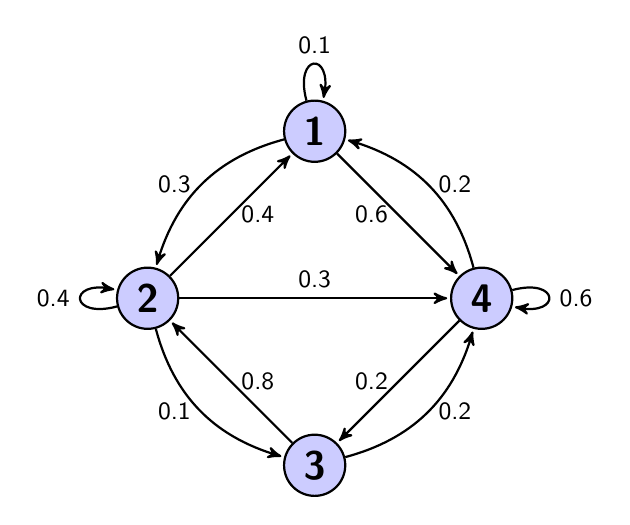
\begin{tikzpicture}[scale=0.75,->,>=stealth',shorten >=1pt,auto,node
    distance=3cm, thick,main
    node/.style={circle,fill=blue!20,draw,font=\sffamily\Large\bfseries}]
    \node[main node] (1) {1};
    \node[main node] (2) [below left of=1] {2};
    \node[main node] (3) [below right of=2] {3};
    \node[main node] (4) [below right of=1] {4};

    \path[every node/.style={font=\sffamily\small}]
    (1) edge node [left] {0.6} (4)
        edge [bend right] node[left] {0.3} (2)
        edge [loop above] node {0.1} (1)
    (2) edge node [right] {0.4} (1)
        edge node {0.3} (4)
        edge [loop left] node {0.4} (2)
        edge [bend right] node[left] {0.1} (3)
    (3) edge node [right] {0.8} (2)
        edge [bend right] node[right] {0.2} (4)
    (4) edge node [left] {0.2} (3)
        edge [loop right] node {0.6} (4)
        edge [bend right] node[right] {0.2} (1);
\end{tikzpicture}
\qquad
\begin{circuitikz}[scale=0.75,american voltages]
\draw
  % rotor circuit
  (0,0) to [short, *-] (6,0)
  to [V, l_=$\mathrm{j}{\omega}_m \underline{\psi}^s_R$] (6,2) % rotor emf
  to [R, l_=$R_R$] (6,4) % rotor resistance
  to [short, i_=$\underline{i}^s_R$] (5,4) % rotor current

  % stator circuit
  (0,0) to [open, v^>=$\underline{u}^s_s$] (0,4) % stator voltage
  to [short, *- ,i=$\underline{i}^s_s$] (1,4) % stator current
  to [R, l=$R_s$] (3,4) % stator resistance
  to [L, l=$L_{\sigma}$] (5,4) % leakage inductance
  to [short, i_=$\underline{i}^s_M$] (5,3) % magnetizing current
  to [L, l_=$L_M$] (5,0); % magnetizing inductance
\end{circuitikz}
  \caption{Un parell de gràfics dissenyats amb tikz.}
  \label{fig:tikz-exemples}
\end{figure}

Hi ha molts altres paquets que permeten treure profit de
\texttt{pgf/tikz} en situacions específiques. Un paquet especialment
interessant és \texttt{pgfplots}, que facilita la generació de gràfics
estadístics i de funcions de molts tipus (histogrames, \est{boxplots},
\est{scatterplots}, etc.). A la figura~\ref{fig:histo}, podeu veure un
exemple del resultat obtingut amb aquest paquet. En aquest cas l'estil
de l'histograma segueix les recomanacions de Tufte
a~\cite{tufte01:_visual_displ_quant_infor}.


\begin{figure}[tbh]
  \centering
  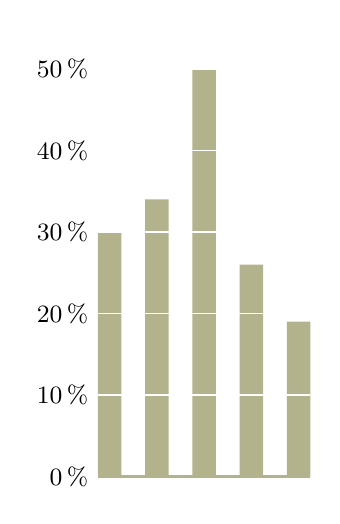
\begin{tikzpicture}[font=\small]
    \begin{axis}[tufte bar]
      \addplot coordinates {
        (1,30)
        (2,34)
        (3,50)
        (4,26)
        (5,19)
      };
    \end{axis}
  \end{tikzpicture}
  \caption{Un histograma dibuixat amb \texttt{pfgplots}.}
  \label{fig:histo}
\end{figure}

\section{Els peus de taula i de figura}

Tant a les taules com a les figures és preceptiu afegir un petit text
que les descriu i que anomenem peu o llegenda. La funció del peu és
semblant a la d'un titular: descriu de manera breu i precisa la imatge
o la taula. No és aconsellable que sigui llarga: una frase o dues com
a molt. Les explicacions i comentaris sobre la figura o la taula s'han
de fer en el text del document.

En alguns casos, el peu pot usar-se per aclarir alguns aspectes de les
imatges. Per exemple, a vegades és útil fer servir una figura formada
per diverses figures petites i el peu pot ajudar a aclarir quin paper
fa cadascuna.

També és corrent que el peu citi la font de la taula o figura. Alguns
estils recomanen fer servir el text «Font: \dots» per indicar d'on
prové el material i, fins i tot, el text «Font pròpia» per indicar que
sou els autors del material. En l'estil del \acro{tfe} es prefereix
evitar aquests textos, que resulten carregosos i repetitius. Quan
siguem els autors d'una figura o d'una taula senzillament no en direm
res: sempre se sobreentén que som els autors del material de la
memòria!. Si, per contra, la taula o la figura l'hem manllevat d'un
altre autor, en el peu citarem la referència de manera natural fent
servir citacions bibliogràfiques (vegeu
l'apartat~\ref{cap:bibliografia}). La manera de fer-ho és afegint en
el mateix peu la citació amb naturalitat com en els següents exemples
de peus: «Diagrama de fases segons [citació]», «Taula de renda
disponible de les comarques centrals d'acord amb [citació]» o
«Fotografia de [citació] en que es pot veure la falla del Tordell».

\chapter{Notació matemàtica}

\LaTeX{} va néixer especialment per escriure textos amb contingut
matemàtic. És molt ric en eines per escriure aquest tipus de material
i està molt documentat a la web. Aquest capítol és una introducció
molt senzilla a aquesta funcionalitat.

El primer que cal saber és que hi ha uns àmbits específics per
escriure terminologia matemàtica. Aquests àmbits es senyalen amb
marques i tot el que queda dins es considera «tipografia matemàtica».

Hi ha dues famílies d'àmbits en que poden aparèixer expressions
matemàtiques:

\begin{enumerate}
\item Dins d'una línia d'un paràgraf ---\est{inline}. En aquest cas
  l'expressió matemàtica s'escriu entre dòlars simples. Per exemple
  \verb!$3\sin^2x$! resulta en $3\sin^2x$ i\break
  \verb!$\int_0^5\frac{1+\tan x}{x}dx$! resulta en
  $\int_0^5\frac{1+\tan x}{x}dx$.
\item Com a part d'un \est{display}, un element que s'escriu en un
  espai propi centrat però no trenca el paràgraf que el conté. En
  aquest cas hi ha diverses maneres de marcar-ho segons la naturalesa
  dels \est{display}. La més senzilla és usar l'entorn definit per les
  marques \verb!\[! i \verb!\]!. Per exemple, les mateixes
  expressions anteriors en aquesta modalitat resulten ser:
  \[
    3\sin^2x
  \]
  i
  \[
    \int_0^5\frac{1+\tan x}{x}dx
  \]
  fixeu-vos que no han trencat el paràgraf en que estem. Més aviat són
  peces que formen part del paràgraf i es presenten centrades en el
  seu interior.
\end{enumerate}

Noteu com la manera en que una formula s'acaba escrivint difereix quan
és \est{inline} de quan és \est{display}. En el primer cas es fan
esforços per que l'alçada de la fórmula no excedeixi l'interlineat,
mentre que en el segon cas els signes prenen la seva mida natural.

Sigui quin sigui l'àmbit, les fórmules s'escriuen amb la mateixa
notació. D'aquesta notació en destaquem el següent:
\begin{itemize}
\item Les claus s'usen per agrupar blocs ---com en un llenguatge de
  programació. Observeu, per exemple, la diferència entre
  \verb!$\sqrt{a}+3$! i \verb!$\sqrt{a+3}$! que resulta en
  $\sqrt{a}+3$ i $\sqrt{a+3}$. Si es volen usar les claus cal
  escapar-les amb una \verb!\! com en aquest exemple
  \verb!$A=\{x|x\in\mathbb{R} \wedge x\geq 10\}$! que resulta en
  $A=\{x|x\in\mathbb{R} \wedge x\geq 10\}$
\item Les funcions ordinàries s'escriuen així: \verb!$\log x$!
  ($\log x$) o \verb!$\sin x$! ($\sin x$). N'hi ha moltes de definides
  que trobareu fàcilment a la web. Aquesta manera d'escriure-les els
  hi dóna la forma apropiada.
\item Per subíndexs i superíndexs es fa servir \verb!_! i \verb!^!
  respectivament. Per exemple, \verb!$x^2$! ($x^2$), \verb!$x^{22}$!
  ($x^{22}$), \verb!$x^{\sin y}_{10}$! ($x^{\sin y}_{10}$).
\item Els «signes grans» també es decoren amb sub i
  superíndexs. Vegeu, per exemple, aquesta fórmula
  \verb!$S=\sum_{i=0}^{i=N}i^2$! que resulta en
  $S=\sum_{i=0}^{i=N}i^2$.
\item Podeu usar lletres gregues ---i altres signes--- pel seu
  nom. Mireu aquestes fórmules: \verb!$R_a = \pi r^2$!
  ($R_a=\pi r^2$), \verb!$\Lambda=\frac{\zeta\cdot\phi}{z^2 + 1}$!
  ($\Lambda=\frac{\zeta\cdot\phi}{z^2 + 1}$), \verb!$A=\overline{B\cup C}$!
  ($A=\overline{B\cup C}$). Trobareu reculls de tots aquests símbols i
  lletres a la web fàcilment.
\end{itemize}

Algunes vegades és convenient numerar els \est{displays} per tal de
poder referenciar posteriorment les fórmules que contenen. A tal
efecte podeu usar l'entorn \texttt{equation}.
\begin{equation}
  \label{eq:llei-pendol}
  l\ddot{\theta} + g\sin\theta = 0
\end{equation}
Això permet citar l'equació des del text i fer notar que
l'Equació~\ref{eq:llei-pendol} descriu el moviment d'un pèndol ideal
de longitud $l$. El \est{display} anterior s'ha escrit d'aquesta
manera:
\begin{verbatim}
\begin{equation}
  \label{eq:llei-pendol}
  l\ddot{\theta} + g\sin\theta = 0
\end{equation}
\end{verbatim}
i el mecanisme d'etiqueta-referència és el mateix que ja s'ha explicat
a l'apartat~\ref{apa:etiquetes}.


\chapter{Algoritmes i programes}

L'àmbit natural de l'enginyeria de sistemes \acro{tic}, fa molt
habitual haver de treballar amb material relacionat amb els
algoritmes, els llenguatges de programació o els intèrprets
d'ordres. Aquesta qüestió resulta especialment dificultosa pel que fa
a mantenir una coherència ortotipogràfica. En aquest capítol s'hi
desgranen alguns punts fonamentals.


\section{Fitxers, ordres i \est{shell}}

En moltes memòries és freqüent haver-se de referir a fitxers concrets
dins del text. Els fitxers ---o directoris o \est{paths}--- s'escriuen
amb lletra «de màquina d'escriure». Per fer-ho compteu amb la macro
\verb|\fitx|, que us permet escriure coses com \fitx{modul.c},
\fitx{/etc/cron.daily/logrotate}, \fitx{~/.config/back%/_window.txt} o
\fitx{~/.bashrc}. Noteu que la macro
tracta correctament els caràcters especials i talla les línies allí on
és apropiat.

Altres vegades és interessant poder parlar d'ordres de l'intèrpret. A
tal efecte usem la macro \verb|\ord|. Per exemple, escrivim
\verb+\ord|pdflatex tfe.tex|+ per a dir que aquest document s'obté
fent \ord|pdflatex tfe.tex|. Noteu que en comptes de les claus aquí
obrim i tanquem l'expressió amb un caràcter qualsevol ---en aquest cas
la barra vertical.



\section{Algoritmes}

En una memòria no és escaient incloure grans llistats de programes o
taules de dades. El lloc escaient per a aquest material és més aviat
en un apèndix i, preferiblement, un suport informàtic accessible des
d'Internet. Això no obstant, sovint és convenient descriure algoritmes
que tenen un paper important en el treball, ja sigui per i\l.lustrar
una idea o per poder-los comentar.  En cas de voler escriure
algoritmes, un paquet especialment útil és \verb!algorithm2e!. Aquest
paquet, que esta ben documentat, permet escriure algoritmes usant una
notació habitual. Si, per exemple, escrivim un algoritme amb aquesta
sintaxi:

\begin{verbatim}
\begin{algorithm}
  \KwIn{$n,m$ dos nombres naturals}
  \KwOut{$r$ el màxim comú divisor d'$n$ i $m$}
  \BlankLine
  \While{$n\neq m$}{
    \eIf{$n>m$}{
      $n := n - m$\;
    }{
      $m := m - n$\;
    }
  }
  $r := m$\;
  \caption{Algoritme d'Euclides}
  \label{alg:euclides}
\end{algorithm}
\end{verbatim}

Obtenim un algoritme dins d'un objecte flotant, com si fos una figura,
similar al que podeu veure en la figura~\ref{alg:euclides}. Per
simplificar l'estructura de la memòria s'ha decidit numerar els
algoritmes en la mateixa llista que les figures ordinàries.

\begin{algorithm}
  \KwIn{$n,m$ dos nombres naturals}
  \KwOut{$r$ el màxim comú divisor d'$n$ i $m$}
  \BlankLine
  \While{$n\neq m$}{
    \eIf{$n>m$}{
      $n := n - m$\;
    }{
      $m := m - n$\;
    }
  }
  $r := m$\;
  \caption{Algoritme d'Euclides}
  \label{alg:euclides}
\end{algorithm}



\chapter{Gestió de la bibliografia}
\label{cap:bibliografia}

\section{Citacions i bibliografia en el \acro{tfe}}

La bibliografia en un document científic, com la memòria d'un
\acro{tfe}, intervé en dos àmbits diferents:
\begin{enumerate}
\item Per un costat en el text principal es fan \emph{citacions} dels
  diferents documents que composen la bibliografia. Aquestes citacions
  permeten molt joc. Algunes formes i usos tradicionals són el
  següents:
  \begin{enumerate}
  \item Citar l'origen d'una informació.

    Sovint es creu que copiar idees d'altres autors i usar-les en un
    treball científic és erroni. Res més lluny de la realitat. No hi
    ha cap problema a fer-ho sempre que se citi el document
    original. Alguns modismes corrents per fer això són, per exemple:

    \begin{quote}
      «D'acord amb Stevens,
      \cite{thurston01:_histor_growt_steam_engin}, la màquina de vapor
      va ser inventada per James Watt.»
    \end{quote}

    \begin{quote}
      «La màquina de vapor va ser inventada per James Watt,
      \cite{thurston01:_histor_growt_steam_engin}.»
    \end{quote}

  \item Basar-se en la feina feta per altres autors.

    Per exemple usant la mateixa notació, vocabulari, fórmula,
    etc. Alguns modismes que podeu fer servir en aquests casos podrien
    ser:

    \begin{quote}
      «Per calcular el rendiment d'una màquina de vapor aplicarem les
      fórmules que indica Thurston a
      \cite{thurston01:_histor_growt_steam_engin}.»
    \end{quote}

    \begin{quote}
      «En aquest capítol farem servir la classificació de les màquines
      de vapor que es defineix a
      \cite{thurston01:_histor_growt_steam_engin}.»
    \end{quote}


  \item Indicar on es pot trobar més informació.

    Això permet al lector ampliar la informació sobre un determinat
    tema que pot complementar el que s'està explicant. Alguns modismes
    habituals són:

    \begin{quote}
      «Per a més informació sobre les màquines de vapor consulteu el
      llibre de Thurston, \cite{thurston01:_histor_growt_steam_engin}.»
    \end{quote}

    \begin{quote}
      «A~\cite{thurston01:_histor_growt_steam_engin} podeu trobar
      informació complementària sobre les màquines de vapor.»
    \end{quote}

  \end{enumerate}

\item Per un altre costat, en un capítol al final del document i abans
  dels apèndix s'hi fa constar una taula amb totes les referències que
  s'han citat en el text degudament ordenades i escrites. En aquesta
  taula, cada document es referencia d'una forma precisa que depèn del
  tipus de document: llibre, article, llei, etc. A més cada referència
  se sol acompanyar d'una etiqueta que correspon a la manera en com
  s'ha citat en el text. El capítol que conté la taula de referències
  el titulem «Bibliografia» i no es numera. Vegeu en aquest mateix
  document la bibliografia al final de la primera part.
\end{enumerate}

La forma de citar una referència i la forma d'escriure una referència
segons el tipus de document segueixen regles estrictes i sofisticades
que es coneixen com «estils de bibliografia». Alguns estils habituals
són APA, \cite{association20:_public_americ_psych_assoc}, \est{Chicago
  Manual of Style}, \cite{chicago17:_chicag_manual_style}, la norma
\acro{iso} 690, \cite{iso21:_iso_690}, o \acro{ieee},
\cite{periodicals18:_ieee_refer_guide} . En el format del \acro{tfe}
apliquem la norma estàndard de BibTeX amb citacions de tipus
alfanumèric, \cite{lehman14:_biblat_packag}.



\section{Eines \LaTeX{} per la bibliografia}

Gestionar la bibliografia no és senzill. Per treballar en aquest àmbit
\LaTeX{} ofereix un conjunt d'eines que faciliten enormement la
tasca. Aquestes eines tenen grans possibilitats però aquí només
en farem una introducció senzilla. Per a més informació
consulteu~\cite{lehman14:_biblat_packag}.

La idea de treball és la següent: en un fitxer (en el nostre cas
\fitx{tfe.bib}) es descriuen les característiques dels documents que
anem citant (nom dels autors, data, etc.). Cada tipus de document té
la seva fitxa i necessita uns camps concrets, alguns obligats i altres
opcionals. Els tipus de documents existents, els camps de cadascun i
el format d'aquests camps poden consultar-se a
\cite[][cap.~2]{lehman14:_biblat_packag}. Aquest fitxer és la
\emph{base de dades bibliogràfica}. Noteu que \texttt{emacs} té un
mode específic per treballar amb aquestes bases de dades. A
l'apèndix~\ref{ape:emacs} trobareu una petita explicació.

En el cas d'aquest exemple, el fitxer \fitx{tfe.bib} conté aquest text
(a més d'altres fitxes bibliogràfiques que s'usen en aquesta
documentació):
\begin{verbatim}
@Book{thurston01:_histor_growt_steam_engin,
  author = {Robert Henry Thurston},
  title = {A History of the Growth of the Steam-Engine},
  publisher = {D. Appleton {and} company},
  year = 1901,
  address = {New York, USA},
  edition = {4th revised},
  langid = {english},
}


@Manual{lehman14:_biblat_packag,
  title = {The Biblatex Package},
  subtitle = {Programmable Bibliographies and Citations},
  author = {Philipp Lehman and Philip Kime and Audrey Boruvka and Joseph Wright },
  version = {2.9a},
  month = 6,
  year = 2014,
  url = {http://mirrors.ctan.org/macros/latex/contrib/biblatex/doc/biblatex.pdf}}
\end{verbatim}

Noteu que al principi de cada entrada hi ha una etiqueta arbitrària
que identifica cada document de la base de dades. Aquesta etiqueta
serveix justament per referenciar el document quan és necessari usant
la construcció \verb|\cite{lehman14:_biblat_packag}|.

En el document corresponent al \acro{tfe} cal indicar quina és la base de
dades que s'usarà escrivint al principi la macro
\verb|\addbibresource{tfe.bib}|. A més, en el lloc on volem que
aparegui la taula de bibliografia cal indicar-ho amb la macro
\verb|\printbibliography|. Normalment la bibliografia apareix després
del darrer capítol del \acro{tfe} i abans dels apèndix si n'hi ha. No
s'acostuma a numerar atès que no forma part del cos del treball com
passa amb els resums i el sumari.  Si consulteu el font d'aquest
exemple podreu apreciar aquesta estructura.

\section{Processat de la bibliografia}

Per processar un document que conté bibliografia cal seguir algun pas
més del que es fa quan només té continguts ordinaris. La seqüència per
compilar aquest mateix exemple, posem per cas, és:
\begin{enumerate}
\item Processeu el document per primer cop fent \ord|pdflatex tfe.tex|.
\item Extraieu les dades que el document necessita per confegir la
  bibliografia de la base de dades bibliogràfica fent \ord|biber tfe|.
\item Processeu de nou el document per incloure les dades
  bibliogràfiques extretes anteriorment fent de nou
  \ord|pdflatex tfe.tex|.
\end{enumerate}

En general cal repetir el segon pas únicament quan es modifica la base
de dades bibliogràfica, ja sigui perquè s'han afegit noves entrades o
perquè s'han corregit entrades existents.


\section{Alguns detalls sobre la bibliografia}
\label{sec:alguns-detalls-sobre}

En aquest apartat s'aclareixen algunes qüestions recurrents
relacionades amb la bibliografia dels \acro{tfe}.

Una pregunta freqüent respecte la bibliografia és: com pot afegir-se
una referència bibliogràfica a la taula de referències sense que hi
hagi una citació a la memòria? La resposta curta és que no s'ha de
fer. Es considera mala praxis referenciar documents que no s'han citat
abans a la memòria. Si un document és rellevant pel \acro{tfe}, segur
que és convenient citar-lo en un o més punts de la memòria!

Els documents tenen diferents graus de rigor\footnote{Aquí «rigor»
  denota el valor que se li pot donar al que diu el document. En certa
  forma és la seva credibilitat.}. Per exemple, una article en una
revista científica reconeguda és una referència amb molt més rigor que
una referència a una pàgina web d'autor desconegut. En el moment de
cercar una referència, sempre preferirem el document més rigorós
possible. Aquesta és una qüestió rellevant en la bibliografia del
\acro{tfe} i cal prestar-hi atenció.






\chapter{Organització de la memòria}

Per organització de la memòria entenem la forma en com s'estructura el
manuscrit en capítols, apartats, annexos, etc.

L'organització de la memòria sempre té com a primer objectiu
transmetre de la millor manera possible la tasca que s'ha dut a
terme. Així, la seva organització serà diferent segons la naturalesa
del treball. Això no obstant, hi ha algunes pautes generals que és
convenient seguir-les sempre. La normativa de \acro{tfe},
\cite{manresa23:_normat_trebal_fi_estud_epsem}, estableix també una
organització per a la memòria que aquest estil respecta. L'estil
\texttt{tfgitic} formata automàticament molts dels elements
d'estructura que són obligats i deixa llibertat en aquells que depenen
del treball concret.

Com s'ha dit a l'apartat~\ref{sec:documentacio}, els fitxers
\fitx{tfe.tex} i \fitx{tfe.bib} són plantilles que apliquen a la
memòria del \acro{tfe} i segueixen l'organització que s'explica en
aquest apartat.


\section{Consideracions generals}

Pel que fa a com organitzar la memòria hi ha nombroses consideracions
a fer que s'han obviat atès que la classe \texttt{tfgitic} ja les té
en compte automàticament.

La memòria té en primera instància dos blocs: el bloc inicial i el bloc
central.
\begin{enumerate}
\item El bloc inicial el conformen la portada, copyright, dedicatoria,
  agraïments, declaració responsable, resums i índex. La manera en com
  es composen i paginen és automàtica.
\item El bloc central el composen els capítols principals de la
  memòria, la bibliografia i els apèndixs si n'hi ha.

  L'estructura organitzativa del bloc central depèn de si hi ha o no
  apèndixs. \emph{Si hi ha apèndix, aleshores es divideix el bloc
    central en dues parts: memòria i apèndixs; en cas que no hi hagi
    apèndixs s'evita la divisió en parts}. La memòria i els apèndix
  els dividim en capítols, apartats, subapartats, i excepcionalment
  subsubapartats.
\end{enumerate}

\section{Divisions principals}

Aquest apartat enumera en l'ordre que apareixen a la memòria les
divisions principals i, quan escau, explica breument quin contingut
han de tenir i a quin objectiu serveixen. També es diu si han de
formar part obligatòriament de la memòria o no.

\subsection*{Bloc de portada}

\begin{enumerate}

\item \emph{Portada} [Obligatori]\par
  La memòria ha de començar amb una portada normativa. Els elements
  que conté s'indiquen abans de bloc \texttt{document} fent servir les
  macros descrites més endavant. Algunes d'aquestes macros permeten
  indicar el gènere i el número del text. Per fer-ho, usen un
  paràmetre opcional amb aquest significat:
  \begin{description}
  \item[m] Masculí singular.
  \item[M] Masculí plural.
  \item[f] Femení singular.
  \item[F] Femení plural.
  \end{description}
  D'aquesta manera, si el \acro{tfe} té una tutora, podem definir els
  seu nom fent:
\begin{verbatim}
\counselor[f]{Adele Goldberg}
\end{verbatim}
  si, en canvi, el treball és codirigit per dues directores, haurem de
  definir-les fent:
\begin{verbatim}
\advisor[F]{Margaret Hamilton i Mary Kenneth Keller}
\end{verbatim}
  A totes les macros que admeten gènere o número, l'absència del
  paràmetre opcional equival a \texttt{m}, o sia masculí
  singular. Així, per exemple, aquestes dues definicions de l'autor
  són equivalents:
\begin{verbatim}
\author{Berenguer de Cruïlles}
\author[m]{Berenguer de Cruïlles}
\end{verbatim}

  La llista de macros que permeten definir les metadades és aquesta:
  \begin{description}
  \item[title] El títol de la memòria. Ha de ser el títol que es va
    enregistrar. És obligatori. Es poden separar línies amb \verb!\\!.
  \item[subtitle] El subtítol de la memòria. És optatiu.
  \item[author] L'estudiant autor del treball. Escrit com a «nom i
    cognoms» i no pas com «cognoms, nom». És obligatori. Admet un
    paràmetre opcional amb un d'aquests valors \texttt{[m|f]}.
  \item[advisor] El director o directors del treball.  Escrit com a
    «nom i cognoms» i no pas com «cognoms, nom». És obligatori. Admet
    un paràmetre opcional amb un d'aquests valors \texttt{[m|M|f|F]}.
  \item[company] L'empresa o institució on es fa el treball quan
    oficialment és fa sota un conveni de pràctiques (modalitat
    «empresa»). És obligat si el treball es fa en modalitat «empresa».
  \item[counselor] El tutor del treball. Quan el treball es fa
    oficialment sota un conveni de pràctiques (modalitat «empresa»),
    el director és una persona de l'empresa. En aquest cas cal que hi
    hagi un tutor, que és un professor amb un rol determinat per la
    normativa, \cite{manresa23:_normat_trebal_fi_estud_epsem}. Escrit
    com a «nom i cognoms» i no pas com «cognoms, nom». És obligatori
    si el treball és de modalitat «empresa». Admet un paràmetre
    opcional amb un d'aquests valors \texttt{[m|f]}.
  \item[location] La ciutat on es defensa el \acro{tfe}. Per omissió
    és Manresa.
  \item[degree] Els estudis. Per omissió el grau d'enginyeria en
    Sistemes TIC (o la seva denominació oficial en anglès si aquesta
    és la llengua de la memòria).
  \item[ects] La càrrega en \acro{ects} del treball. Per omissió és la
    càrrega del grau d'enginyeria en Sistemes TIC, és a dir 24.
  \item[school] L'escola. Per omissió l'Escola Politècnica Superior
    d'Enginyeria de Manresa (o la seva denominació oficial en anglès
    si aquesta és la llengua de la memòria).
  \item[topics] Els dos àmbits temàtics principals en que s'emmarca el
    treball, d'acord
    amb~\cite{manresa23:_normat_trebal_fi_estud_epsem}. Els àmbits els
    determina el director (o el tutor en el seu cas) i els escull
    d'una llista tancada que estableix el procediment del \acro{tfe}.
  \end{description}

\item \emph{Dedicatòria i agraïments} [Optatiu]\par
  La memòria pot contenir si escau una dedicatòria i/o uns
  agraïments. La dedicatòria ha de ser breu i s'escriu emprant la macro
  \verb|\dedication|. Els agraïments han d'allargar-se entre un tres
  paràgrafs i s'escriuen en l'entorn
  \verb|acknowledgments|. Automàticament se situen on cal en cas
  d'emprar-se.

\item \emph{Resums} [Obligatori]\par
  L'objectiu del resum és que el lector pugui conèixer ràpidament el
  propòsit i les conclusions del treball, en definitiva per què el
  treball és interessant. No ha de passar de mitja pàgina.

  És obligat escriure un resum en català i un altre en anglès. Els
  resums s'escriuen abans del bloc \verb!document! cadascun en un
  entorn específic. La classe \texttt{tfgitic} els formata i situa
  convenientment dins del document. Els entorns són:

  \begin{description}
  \item[resum] Pel resum en català.
  \item[abstract] Pel resum en anglès.
  \end{description}

\item \emph{Índex} [Obligatori]\par
  És automàtic.
\end{enumerate}

\subsection*{Bloc central}

\subsubsection*{Part I: Memòria}

\begin{enumerate}\setcounter{enumi}{4}

\item \emph{Introducció} [Obligatori]\par
  És un capítol obligatori. La seva funció és explicar al lector que
  es trobarà en la memòria. Alguns elements ---que a vegades prenen
  forma d'apartats--- que han de sortir-hi són:
  \begin{enumerate}
  \item El context en què se situa el treball, la descripció dels
    seus objectius i el seu interes argumentat.
  \item Els resultats que s'han obtingut.
  \item Si n'hi ha, les circumstàncies que poden limitar la
    realització del treball. Per exemple, el material disponible o
    el pressupost amb que es compta per comprar material.
  \item L'enumeració dels objectius concrets.
  \item L'organització de la memòria, en què s'explica al lector
    quin és el fil conductor del manuscrit i què es trobarà quan
    continuï llegint.
  \end{enumerate}

  Una altre funció rellevant de la introducció és seduir al lector per
  a què s'interessi pel treball. El lector s'ha de quedar amb la
  sensació de què el treball és interessant, ha de tenir ganes de
  continuar llegint.

\item \emph{Antecedents} [Obligatori]\par
  És el capítol dedicat a donar al lector tota la informació prèvia
  que necessitarà per entendre el treball. Típicament són dos tipus
  de coses:
  \begin{itemize}
  \item Treballs que altres persones han fet en el mateix
    àmbit. Sovint s'exposen d'una manera endreçada amb la intenció que
    el lector acabi tenint una bona perspectiva de l'àmbit en què se
    situa el treball. És el espai escaient per criticar i comparar
    altres treballs sobre el mateix tema si escau.
  \item Coneixements sobre teories, eines, llenguatges, notacions,
    etc. que juguen un paper instrumental en el desenvolupament del
    treball
  \end{itemize}
  El capítol no ha de ser un llibre sinó una breu exposició. És
  interessant aportar referències que permetin al lector aprofundir
  més en algun dels aspectes, si li interessa, al mateix temps que
  s'indiquen les fonts d'on s'ha obtingut la informació.

\item \emph{Cos del treball} [Obligatori]\par
  Són els capítols en què s'explica el treball. El seu nombre i
  organització depenen de cada treball en concret i no es poden
  generalitzar.

\item \emph{Estudi econòmic} [Optatiu]\par
  En el cas que el treball ho requereixi, aquest capítol desenvolupa
  els aspectes econòmics relacionats amb el treball.

\item \emph{Impacte ambiental i social} [Optatiu]\par
  En el cas que el treball ho requereixi, aquest capítol elabora els
  aspectes relacionats amb l'impacte ambiental relacionats amb el
  treball.

\item \emph{Conclusions} [Obligatori]\par
  En el capítol de conclusions cal resumir els resultats del
  treball. Cal emfasitzar els resultats més importants i
  relacionar-los amb els objectius que es tenien.

  També és l'apartat escaient per indicar els objectius que no s'han
  assolit i reflexionar sobre per què no s'han assolit.

\item \emph{Treball futur} [Optatiu]\par
  Si cal es pot afegir un capítol sobre «treball futur» en el que es
  desgranin aquelles línies de treball que podrien ser continuació
  natural del treball. És convenient exposar, com a molt, només les
  tres o quatre més importants. S'han d'explicar, situar en el marc
  del treball i suggerir breument algunes idees sobre com es podrien
  encarar.

\item \emph{Bibliografia} [Obligatori]\par
  Capítol especial, no numerat, que conté les referencies de totes les
  obres citades en el manuscrit. Tot i que la seva composició és
  complexa, la feina la fa íntegrament el gestor de referències i no
  cal preocupar-se'n especialment. Vegeu el
  capítol~\ref{cap:bibliografia} a la pàgina~\pageref{cap:bibliografia}.

\end{enumerate}

\subsubsection*{Part II: Apèndixs}

\begin{enumerate}\setcounter{enumi}{12}

\item \emph{Apèndixs} [Optatiu]\par
  En certs casos podria ser interessant que la memòria del \acro{tfe}
  tingui un o més apèndixs.

  Quan hi ha materials o dades que es fan servir per donar suport a un
  capítol però són massa llargs o massa detallats per a ser inclosos
  en la memòria, es consignen en un apèndix i es referencien des dels
  capítols principals.

  Aquest tipus de material complementari canvia segons el
  treball. Alguns exemples típics són:
  \begin{itemize}
  \item Taules de dades.
  \item Mapes o plànols.
  \item Exemples de formularis emprats en una enquesta.
  \item Documents (parts de) citats en el treball que són difícils de
    trobar.
  \item Transcripcions de converses o gravacions.
  \item Programes informàtics.
  \end{itemize}

  Tingueu en consideració que, com a norma general, tot aquell
  material que pot ser referenciat és preferible consignar-lo com una
  referència i no com un apèndix.

  En el cas que necessiteu apèndixs, cal organitzar el document en
  dues parts: la memòria pròpiament i els apèndixs. Aquesta mateixa
  documentació n'és un exemple. Contràriament, si no necessiteu cap
  apèndix és millor que no subdividiu la memòria en
  parts. Senzillament heu de treure les macros \verb!\part{}!.

\end{enumerate}


\printbibliography


\appendix

\part{Apèndixs}

\chapter{Regles d'or de la memòria de TFE}

\colorbox{yellowmarker}{
  \begin{minipage}{1.0\linewidth}
    \Large\sffamily
    \begin{enumerate}
    \item Mai s'han de forçar salts de pàgina, afegir o treure espai
      aquí o allà, canviar la lletra, o qualsevol altre canvi de
      forma. Deixeu que la forma la determini \LaTeX{} i preocupeu-vos
      pel contingut.
    \item El text i allò que explica és la part central de la vostra
      memòria de TFE. El vostre document no és una revista, ni
      un catàleg, ni un pasquí publicitari.
    \item Les figures són per ajudar a entendre allò que s'explica en
      el text. Afegir figures «per omplir» la memòria o «per que n'hi ha
      d'haver» o per que «fan maco» és inapropiat. Trieu
      estrictament les figures que fan falta i dissenyeu-les
      acuradament per que compleixin la seva funció. Pregunteu-vos què
      passaria si una figura la traieu; si allò què voleu explicar no
      se'n ressent, és una figura sobrera.
    \item Useu les figures flotants i no en fixeu la seva posició. Si
      el nombre de figures és l'escaient, el mecanisme de posicionat
      flotant situarà les figures a la millor posició.
    \item Referencieu les figures des del text i arrepenjeu-vos-hi per
      explicar millor allò que us interessa transmetre.
    \item Trieu referències bibliogràfiques de bona qualitat. Eviteu
      citar pàgines web d'institucions sense autoritat, d'institucions
      amb interessos publicitaris o material de divulgació.
    \item Treballeu amb referències bibliogràfiques completes. Feu que
      hi consti tota la informació disponible sobre el document. Les
      referències bibliogràfiques incompletes s'han d'estalviar.
    \item Feu que les citacions en el text en reforcin el discurs,
      ampliïn el seu abast i deixin clara l'autoria de les idees
      d'altri.
    \end{enumerate}
    \smallskip
  \end{minipage}
}


\chapter{Història d'aquesta classe}
\label{cap:historia}

\begin{tabularx}{\textwidth}{lX}
  \toprule
  Versió  & Modificacions \\
  \midrule
  %current version
  7.1 & Actualització de les versions mínimes d'alguns
  paquets. Millores en la i18n.  Afegit gènere/número a les macros
  sobre persones. Millores en la partició de mots
  en català. Missatges d'error per a combinacions impròpies de metadades.
  Reflecteix informació tipogràfica a la cara parell de la portada.
  Correcció d'errates caçades per Aleix Llusà.\\
  7.0 & Correcció d'errors caçats per Èric Roy. Actualització a la
  versió vigent del paquet \texttt{siunitx}. Afegit apartat sobre peus
  de figura i de taula. Afegida la «declaració responsable» que
  requereix la normativa de plagi. Diferenciats els rols de
  tutor/director. Afinada la denominació del treball segons
  grau/màster. Modificada la nomenclatura \acro{tfg} al més general
  \acro{tfe}. Opció per determinar si és \acro{tfe} de grau o
  màster. Solucionat error en numeració de pàgines.\\
  6.5 & Millores del sistema de releasing.\\
  6.4 & Errates. Actualització del logo \acro{upc} d'acord amb la
  normativa actual. En la documentació, afegida l'ordre \texttt{C-c
    C-a} d'\texttt{AUCTeX}. Actualitzada la llicència \acro{cc} a la
  versió 4.0. Els entorns \texttt{resum} i \texttt{abstract}
  assumeixen l'ortotipografia de la llengua corresponent i respecten
  els paràgrafs. Afegida la població a la portada. Afegits alguns
  comentaris sobre la bibliografia. L'entorn \texttt{summary} passa a
  \texttt{abstract}. Actualització de la bibliografia.
  Generalitzat per a ser usable en altres títols i escoles.\\
  6.3 & Errates. Avenços significatius en les eines de releasing.
  Modificat i documentat escriptura magnitud enteres.  Corregit error
  en implementació abstracts: no reconeixia
  paràgrafs. \\
  6.2 & Petites millores a la documentació.\\
  6.1 & Eliminats warnings menors. Versionat de la
  classe \texttt{tfgitic}.\\
  6 & La documentació incorpora annexos sobre \LaTeX{} i
  \texttt{emacs}. Capítol sobre escriptura d'expressions
  matemàtiques. Corregit nom de l'escola en la memòria .\\
  5 & La classe suporta anglès i català. Millorada portada. Afegits
  agraïments.
  Documentació més extensa. Nou apartat sobre organització de la memòria.\\
  4 & Tractament de cometes automàtic i preparat per a l'anglès.\\
  3 & Bibliografia surt a l'índex.\\
  2 & Afegida macro opcional pel subtítol.\\
  1 & Afegida història de la classe. Comentari sobre el tall de línia
  en una ela geminada. Nova referència. Refet apartat sobre apèndixs.\\
  \bottomrule
\end{tabularx}


\chapter{Brevíssima introducció a \LaTeX}
\label{ape:intro-latex}

\LaTeX{}, \cite{lamport94:_latex_ed}, és un sistema de composició de
textos de molt alta qualitat. No és un sistema \acro{wysiwyg} sinó que
funciona com un compilador: escrivim el document en «llenguatge font»
i, després de compilar-lo, obtenim un fitxer en format
\texttt{pdf}. \LaTeX{} és, de fet, el llenguatge font. Com a
llenguatge, és de tipus \est{mark-up}. És a dir, escrivim el text i,
quan cal, anem inserint marques que indiquen la categoria del text:
això és un títol, allò és una llista, allò altre és una fórmula,\dots

Aquest és l'avantatge: quan escrivim ens preocupem sobretot dels
continguts i és el compilador que s'encarregarà de donar-li forma
automàticament. La forma que li dóna no és sempre la mateixa: depèn de
la classe de document. Canviant la classe o els seus paràmetres s'obté
un resultat diferent. Aquest document, per exemple, descriu una classe
que formata un document d'acord amb els usos i costums de les memòries
dels \acro{tfe}.

És una regla d'or ---la regla més important--- quan s'escriu un
document \LaTeX{} no intentar contravenir la manera de formatar el
document que estableix la classe. La forma és responsabilitat
exclusiva de la classe.

El font del document s'escriu amb un editor en un fitxer de text. Per
exemple en el fitxer \fitx{docum.tex}. Aquest fitxer podria tenir un
contingut com aquest:

\begin{verbatim}
\documentclass[a4paper,12pt]{article}
\usepackage[catalan]{babel}

\title{Un exemple}
\author{Ramon Gener}

\begin{document}
\maketitle{}

\section{Introducció}
Això és un apartat d'exemple. I això que segueix una \emph{enumeració}:
\begin{enumerate}
\item Primer punt.
\item Segon punt.
\item Tercer punt.
\end{enumerate}
\end{document}
\end{verbatim}

Per compilar-lo es podria fer:
\begin{verbatim}
$ pdflatex docum.tex
\end{verbatim}
després de molts missatges, es genera un fitxer de nom
\fitx{docum.pdf} que és el resultat. A vegades, per raons que ara no
és prudent explicar, amb una sola compilació no n'hi ha prou. Per
simplificar les coses podeu usar l'ordre \ord|latexmk|, que aplica les
vegades que necessàries el compilador. Cal que la insta\l.leu
prèviament fent:
\begin{verbatim}
$ sudo apt install latexmk
\end{verbatim}
L'ordre permet fer algunes tasques habituals mentre treballem amb
\LaTeX{} com ara generar el \texttt{pdf} o esborrar tots els fitxers
auxiliars. A la pàgina de \texttt{man} corresponent hi trobareu els
detalls. Per generar el \texttt{pdf}, per exemple, faríem:
\begin{verbatim}
$ latexmk -pdf docum.tex
\end{verbatim}

Si useu l'editor \texttt{emacs}, cosa que recomanem, feu-li un
cop d'ull a l'apèndix~\ref{ape:emacs}.

Per aprendre els rudiments de \LaTeX{} hi ha moltíssim material on
triar. Una referència que pot ajudar-vos
és~\cite{oetiker:_not_so_short_introd_latex}.


\chapter{Suport d'emacs}
\label{ape:emacs}

\texttt{Emacs},
\cite{foundation19:_gnu_emacs,stallman81:_emacs_exten_custom_self_displ_editor}
, és l'editor recomanat per treballar amb \LaTeX{}. El suport
d'\texttt{emacs} per editar i processar documents \LaTeX{} es fa en
primer terme a través de l'extensió ---\est{plugin}--- anomenada
\texttt{auctex}, \cite{thorup17:_auctex_sophis}, i en segon terme a
través de l'extensió anomenada \texttt{reftex},
\cite{dominik09:_reftex_user_manual}, que co\l.labora amb la primera
per tal de facilitar l'ús de referències i citacions. Les eines de
suport són extenses i inclouen funcions com les següents:
\begin{itemize}
\item Inserció de macros i entorns a «cop de tecla».
\item Formatat automàtic del document font.
\item Acolorit de les estructures per a una millor lectura.
\item Suport al cicle de compilació-visualització.
\item Inserció de cites i referències amb auto-compleció.
\item Manteniment de la base de dades de bibliografia.
\end{itemize}

\section{Insta\l.lació}

Simplement insta\l.leu, si cal, els paquets necessaris fent:
\begin{verbatim}
$ apt-get install emacs
$ apt-get install auctex
\end{verbatim}
i tot seguit editeu el fitxer de configuració d'emacs \fitx{~/.emacs}
afegint al final les següents línies per tal d'activar el mode
\texttt{reftex} sempre que \texttt{auctex} sigui actiu:
\begin{verbatim}
;; turn-on reftex when auctex active
(add-hook 'LaTeX-mode-hook 'turn-on-reftex)
(setq reftex-plug-into-AUCTeX t)
\end{verbatim}

La propera vegada que useu \texttt{emacs} ja tindreu els modes ben
configurats.

\section{Ús bàsic}

Quan editeu un fitxer amb sufix \fitx{.tex} l'editor automàticament
entrarà en «mode latex». En el menú us apareixerà (a) una entrada que
us permet inserir estructures sota el nom de «LaTeX» i (b) una entrada
que us permet compilar i visualitzar el font sota el nom de «Command».
Com és habitual, la majoria d'ordres també estan disponibles com a
combinació de tecles i, sovint, són de més bon fer servir. La
taula~\ref{tab:ordres-emacs} mostra algunes de les combinacions més
emprades. És especialment important l'ordre que va aplicant al
document el procés que li toca en cada moment (\texttt{C-c C-c}).

\begin{table}
  \centering
  \begin{tabularx}{\textwidth}{lX}
    \toprule
    Ordre & Funció \\
    \midrule
    \texttt{C-c C-e} & Insereix un entorn. En alguns casos pregunta pel paràmetres necessaris.\\
    \texttt{C-c C-s} & Insereix una secció, subsecció, capítol, etc.\\
    \texttt{C-c RET} & Insereix una macro. Per exemple \texttt{author}.\\
    \texttt{ALT-RET} & Insereix un nou punt dins d'un entorn de llista
    (\texttt{itemize},
    \texttt{enumerate}, \texttt{description}).\\
    \texttt{C-c [} & Insereix una citació. Suggereix varies
    possibilitats a partir de la base de dades de referències. \\
    \texttt{C-c )} & Insereix una citació. Suggereix varies
    possibilitats a partir de la base de dades de referències. \\
    \texttt{C-c C-c} & Fes el següent procés. Si acabem d'editar
    suggereix compilar el font, si està compilat suggereix
    visualitzar. De manera més o menys elaborada determina quin és el
    següent pas que cal aplicar al document i el fa.\\
    \texttt{C-c C-a} & Processa tot el que calgui i visualitza. Si
    acabem d'editar compila el font, si cal passa \texttt{biber}
    i torna a compilar. És l'ordre que més es fa servir del mode.\\
    \bottomrule
  \end{tabularx}
  \caption{Ordres més habituals d'emacs per treballar amb \LaTeX{}. El
    prefix \texttt{C-} significa control.}
  \label{tab:ordres-emacs}
\end{table}

En cas que el fitxer que editeu sigui una base de dades de
bibliografia, és a dir, tingui sufix \fitx{.bib}, aleshores s'activa
el mode \texttt{bibtex/biblatex}, que permet gestionar aquests fitxers
amb comoditat. Els menús que apareixen us permetran inserir plantilles
per cada tipus de document, per exemple \texttt{@Book}. Les plantilles
insereixen tots els camps possibles. Els que estan prefixats per
\texttt{OPT} són camps optatius. Quan hagueu omplert un camp, salteu
al següent amb l'ordre \texttt{C-j}. Una vegada s'han omplert els
camps apropiats, l'ordre \texttt{C-c C-c} elimina els camps sobrers,
verifica la sintaxi i suggereix una clau d'accés a la referència. Ja
teniu una nova referència a la base de dades!.



\end{document}

%%% Local Variables:
%%% mode: latex
%%% TeX-master: t
%%% LaTeX-biblatex-use-Biber: t
%%% End:
